\chapter{Использование компилятора командной строки и текстового редактора Geany}
\markboth{Приложение А. Использование компилятора командной строки}{Приложение А. Использование компилятора командной строки}

Одним из самых мощных современных кроссплатформенных компиляторов языка \Sys{C++} является свободно-распространяемый
компилятор \Sys{g++}. Для его установки в debian-подобных ОС семейства Linux (Debian, Ubuntu, Mint и их клоны) достаточно
выполнить команду терминала \Sys{apt-get install g++} с правами суперпользователя (администратора) или
воспользоваться менеджером пакетов \Sys{synaptic}.

Установка компилятора \Sys{g++} в ОС семейства Windows несколько сложнее, поэтому  рассмотрим этот процесс более подробно.

\begin{enumerate}
\item На сайте \url{mingw.org} переходим в раздел \Sys{Download} (Загрузки), в появившемся окне щелкаем по ссылке
\Sys{Download mingw-get-setup.exe} (рис.~\ref{app:refDrawing0}). Загружаем установочный файл и запускаем его.
\item На первом этапе установки необходимо выбрать команду \Sys{Install} (см. рис.~\ref{app:refDrawing1}), затем
папку для установки (рис.~\ref{app:refDrawing2}).
\item После этого начнётся процесс доустановки инсталлятора (рис.~\ref{app:refDrawing3}).
\item Далее выбираем компиляторы для установки (\Sys{C++}, \Sys{Fortran}, \Sys{Ada}) (рис.~\ref{app:refDrawing4}) и ждем пока будут
скачаны и установлены необходимые компиляторы. После завершения процесса установки компиляторы (в нашем случае
компилятор \Sys{C++}) готовы к использованию. Но для вызова их (из командной строки Windows, из текстового редактора Geany)
необходимо указывать полное имя файла с компилятором. При установке компилятора \Sys{C++} в стандартный каталог
\Sys{C:{\textbackslash}MinGW} --- полное имя компилятора \Sys{C++} будет таким
\Sys{C:{\textbackslash}MinGW{\textbackslash}bin{\textbackslash}g++}. Для того, чтобы каждый раз не писать полное имя
компиляторы, можно добавить путь  \Sys{C:{\textbackslash}MinGW{\textbackslash}bin} в список путей системной
переменной \Sys{Path}.
\item Для изменения значения системной переменной \Sys{Path} необходимо в панели управления выбрать \emph{Система ->
Дополнительные параметры системы -> Дополнительно -> Переменные среды -> Системные переменные -> Path -> Изменить}. В
открывшемся диалоговом окне добавить путь \Sys{C:{\textbackslash}MinGW{\textbackslash}bin{\textbackslash}}.
\end{enumerate}

\begin{figure}[htb]
\begin{center}
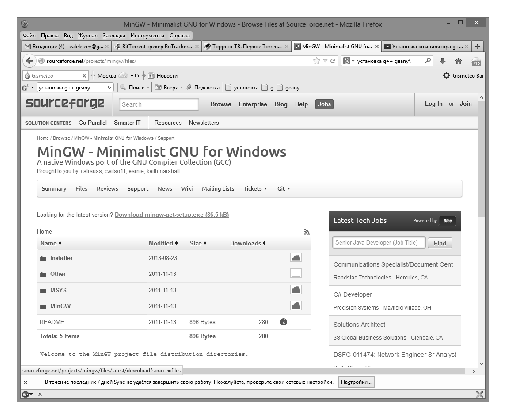
\includegraphics[width=0.7\textwidth]{img/ris_app_1}
\caption[Окно загрузки \Sys{mingw}.]{Окно загрузки \Sys{mingw}.}
\label{app:refDrawing0}
\end{center}
\end{figure}

\begin{figure}[htb]
\begin{center}
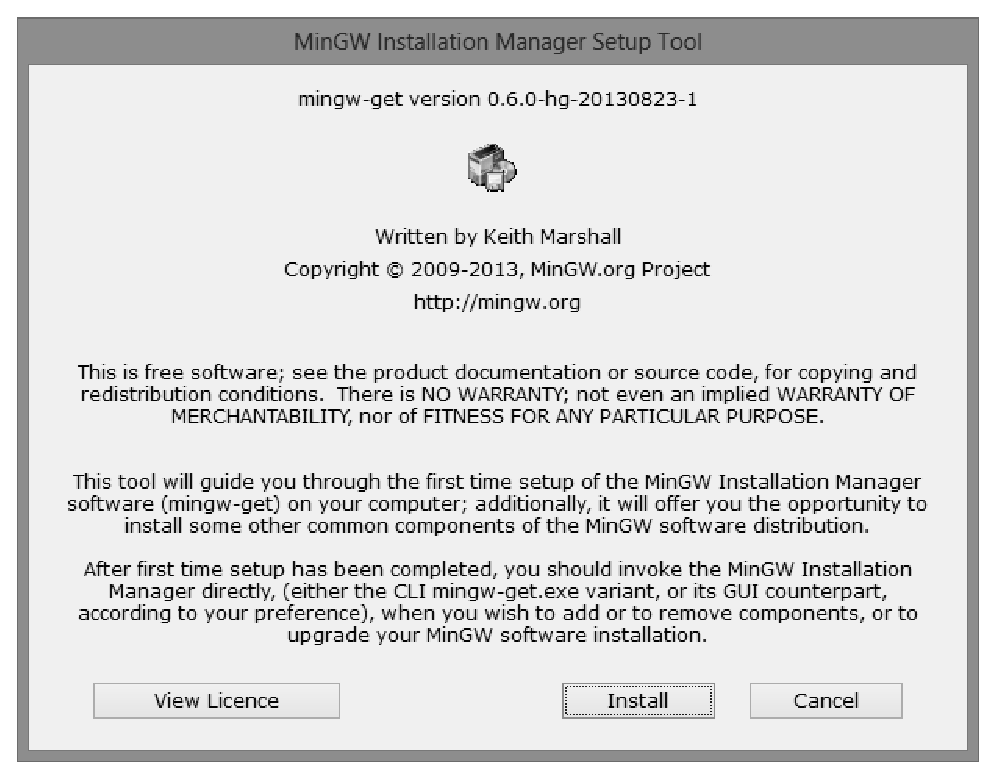
\includegraphics[width=0.7\textwidth]{img/ris_app_2}
\caption[Первое окно установки mingw.]{Первое окно установки mingw.}
\label{app:refDrawing1}
\end{center}
\end{figure}

\begin{figure}[htb]
\begin{center}
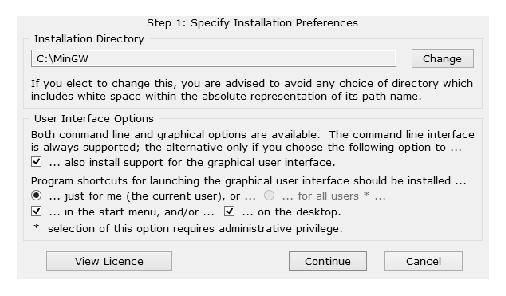
\includegraphics[width=0.7\textwidth]{img/ris_app_3}
\caption[Выбор папки для установка компилятора.]{Выбор папки для установка компилятора.}
\label{app:refDrawing2}
\end{center}
\end{figure}

\begin{figure}[htb]
\begin{center}
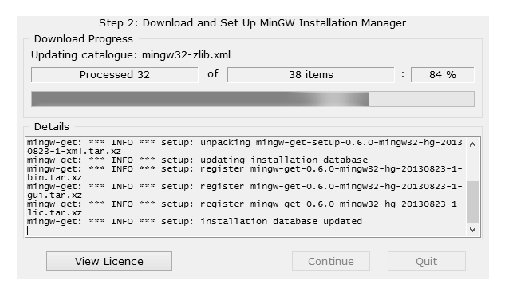
\includegraphics[width=0.7\textwidth]{img/ris_app_4}
\caption[Загрузка инсталлятора.]{Загрузка инсталлятора.}
\label{app:refDrawing3}
\end{center}
\end{figure}


\begin{figure}[htb]
\begin{center}
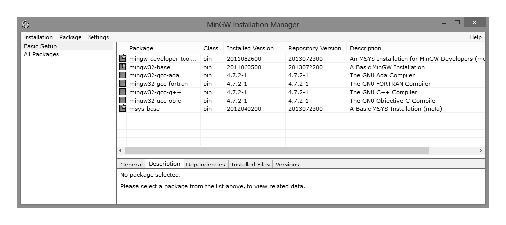
\includegraphics[width=0.7\textwidth]{img/ris_app_5}
\caption[Выбор устанавливаемых компиляторов.]{Выбор устанавливаемых компиляторов.}
\label{app:refDrawing4}
\end{center}
\end{figure}

После перезагрузки ОС Windows для обращения к компилятору достаточно будет указывать его имя --- \Sys{g++}.

Таким образом, в ОС Linux для работы с компилятором в командной строке необходимо запустить Терминал, а в ОС Windows –
командную строку. После чего работа с компилятором \Sys{g++} с ОС Windows и Linux идентична.

Рассмотрим опции компилятора командной строки, необходимые для компиляции и запуска простейших программ. 

Для того, чтобы создать исполняемый файл из текста программы на \Sys{C++}, необходимо выполнить команду 

\Sys{g++ name.cpp} 

Здесь \Sys{name.cpp} --- имя файла с текстом программы. В результате будет создан исполняемый файл со стандартным
именем \Sys{a.out}. Для того, чтобы создать исполняемый файл с другим именем, необходимо выполнить команду 

\Sys{g++ -o nameout name.cpp} 

Здесь \Sys{name.cpp} --- имя файла с текстом программы, \Sys{nameout} --- имя исполняемого файла. 

При использовании компилятора \Sys{g++} после компиляции программы автоматически происходит компоновка программы (запуск
компоновщика make). Чтобы исключить автоматическую компоновку программы следует использовать опцию -c. В этом случае
команда будет иметь вид \Sys{g++ -c name.cpp} 


Технология работы с компилятором \Sys{g++} может быть такой: набираем текст программы в стандартном текстовом редакторе, потом
в консоли запускаем компилятор, после исправления синтаксических ошибок, запускаем исполняемый файл.  После каждого
изменения текста программы, надо сохранить изменения в файле на диске, запустить компилятор, и только после этого
запускать программу (исполняемый файл). Очень важно не забывать сохранять текст программы, иначе при запуске
компилятора будет компилироваться старая версия текста программы. 


Компилятор \Sys{g++} эффективен при разработке больших комплексов программ, он позволяет собирать приложения из нескольких
файлов, создавать библиотеки программ. Рассмотрим процесс создания и использования библиотеки решения задач линейной
алгебры (см. п.~\ref{ch06:4}, задачи~\ref{ch06:prg9} --- \ref{ch06:prg11}):

\lstinline!int SLAU(double **matrica_a,  int n, double *massiv_b, double *x)! --- функция решения системы линейных
алгебраических уравнений;

\lstinline!int INVERSE(double **a, int n, double **y)! --- функция вычисления обратной матрицы;

\lstinline!double determinant(double **matrica_a, int n)! --- функция вычисления определителя.


Для создания библиотеки создадим заголовочный файл \Sys{slau.h} и файл  \Sys{slau.cpp}, в
который поместим тексты всех трёх функций решения задач линейной алгебры.

Текст файла \Sys{slau1.h}:
\begin{lstlisting}
int SLAU(double **matrica_a,  int n, double *massiv_b, double *x);
int INVERSE(double **a, int n, double **y);
double determinant(double **matrica_a, int n);
\end{lstlisting}

Текст файла \Sys{slau1.cpp}:
\begin{lstlisting}
#include <math.h>
int SLAU(double **matrica_a,  int n, double *massiv_b, double *x)
{
   int i,j,k,r;
  double c,M,max,s;
  double **a, *b; 
a=new double *[n];
for(i=0;i<n;i++)
a[i]=new double[n];
b=new double [n];
   for(i=0;i<n;i++)
     for(j=0;j<n;j++)
      a[i][j]=matrica_a[i][j];
   for(i=0;i<n;i++)
     b[i]=massiv_b[i];
    for(k=0;k<n;k++)
  {
    max=fabs(a[k][k]);
    r=k;
    for(i=k+1;i<n;i++)
      if (fabs(a[i][k])>max)
      {
        max=fabs(a[i][k]);
        r=i;
      }
    for(j=0;j<n;j++)
    {
      c=a[k][j];
      a[k][j]=a[r][j];
      a[r][j]=c;
    }
    c=b[k];
    b[k]=b[r];
    b[r]=c;
    for(i=k+1;i<n;i++)
    {
      for(M=a[i][k]/a[k][k],j=k;j<n;j++)
        a[i][j]-=M*a[k][j];
      b[i]-=M*b[k];
    }
  }
  if (a[n-1][n-1]==0)
    if(b[n-1]==0)
      return -1;
    else return -2;
  else
  {
    for(i=n-1;i>=0;i--)
    {
      for(s=0,j=i+1;j<n;j++)
        s+=a[i][j]*x[j];
      x[i]=(b[i]-s)/a[i][i];
    }
    return 0;
  }  
}
int INVERSE(double **a, int n, double **y)
{
  int i,j,res;
  double *b, *x;
  b=new double [n];
  x=new double [n];
  for(i=0;i<n;i++)
  {
    for(j=0;j<n;j++)
      if (j==i)
        b[j]=1;
      else b[j]=0;
      res=SLAU(a,n,b,x);
      if (res!=0) 
        break;
      else
        for(j=0;j<n;j++)
          y[j][i]=x[j];
  }
  if (res!=0)
    return -1;
  else
    return 0;
}
double determinant(double **matrica_a, int n)
{
   int i,j,k,r;
  double c,M,max,s,det=1;
  double **a; 
  a=new double *[n];
  for(i=0;i<n;i++)
    a[i]=new double[n];
  for(i=0;i<n;i++)
    for(j=0;j<n;j++)
      a[i][j]=matrica_a[i][j];
  for(k=0;k<n;k++)
  {
    max=fabs(a[k][k]);
    r=k;
    for(i=k+1;i<n;i++)
      if (fabs(a[i][k])>max)
      {
        max=fabs(a[i][k]);
        r=i;
      }
      if (r!=k) det=-det;
    for(j=0;j<n;j++)
    {
      c=a[k][j];
      a[k][j]=a[r][j];
      a[r][j]=c;
    }
    for(i=k+1;i<n;i++)
      for(M=a[i][k]/a[k][k],j=k;j<n;j++)
        a[i][j]-=M*a[k][j];
  }
  for(i=0;i<n;i++)
    det*=a[i][i];
  return det;
  for(i=0;i<n;i++)
    delete [] a[i];
  delete [] a;
}
\end{lstlisting}


В качестве тестовой задачи напишем главную функцию, которая предназначена для решения системы линейных алгебраических
уравнений.
\begin{lstlisting}
#include <iostream>
#include <math.h>
//`Подключение личной библиотеки \Sys{slau}`
#include "slau1.h"
using namespace std;
int main()
{
  int result,i,j,N;
  double **a, *b, *x; 
  //`Ввод размерности системы.`
  cout<<"N=";
  cin>>N;
  //`Выделение памяти для матрицы правых частей и вектора свободных членов.`
  a=new double *[N];
  for(i=0;i<N;i++)
    a[i]=new double[N];
  b=new double [N];
  x=new double [N];
  //`Ввод матрицы правых частей и вектора свободных членов`.
  cout<<"Input Matrix A"<<endl;
  for(i=0;i<N;i++)
    for(j=0;j<N;j++)
      cin>>a[i][j];
  cout<<"Input massiv B"<<endl;
  for(i=0;i<N;i++)
    cin>>b[i];
  //`Вызов функции решения СЛАУ методом Гаусса из библиотеки \Sys{slau.h}`
  result=SLAU(a,N,b,x);
  if (result==0)
  {
  //`Вывод массива решения.`
  cout<<"Massiv X"<<endl;
  for(i=0;i<N;i++)
    cout<<x[i]<<"\t";
  cout<<endl;
  }
  else if (result==-1)
    cout<<"`\Sys{Бесконечное множество решений}`\n";
    else if (result==-2)
      cout<<"`\Sys{Нет решений}`\n";
}
\end{lstlisting}

Теперь необходимо из этих текстов создать работающее приложение. Рассмотрим это поэтапно.

\begin{enumerate}
\item Компиляция библиотеки \Sys{slau1.h} с помощью команды \Sys{g++ -c slau1.cpp}.
\item Компиляция главной функции \Sys{main.cpp} с помощью команды \Sys{g++ -c main.cpp}.
\item Создание исполняемого файла с именем \Sys{primer} из двух откомпилированных файлов \Sys{main.o} и
\Sys{slau1.o} с помощью команды \Sys{g++ main.o slau1.o -o primer}.
\item Запуск исполняемого файла.
\end{enumerate}
После разработки библиотеки линейной алгебры пример \Sys{slau1}, можно использовать её в различных программах при
вычислении определителя, обратной матрицы и решения систем линейных алгебраических уравнений.

При разработке программ с большим количеством вычислений, компилятор \Sys{g++} позволяет оптимизировать программы по
быстродействию. Для получения оптимизированных программ можно использовать ключи \Sys{-O0}, \Sys{-O1},
\Sys{-O2}, \Sys{-O3}, \Sys{-Os}:

\begin{itemize}
\item при использовании ключа \Sys{-O0} оптимизация отключена, достигается максимальная скорость компиляции, опция
задействована по умолчанию;
\item при использовании ключа <<мягкой>> оптимизации \Sys{-O1} происходит некоторое увеличение времени
компиляции, этот ключ оптимизации позволяет одновременно уменьшать занимаемую программой память и уменьшить время
выполнения программы;
\item при использовании ключа \Sys{-02} происходит существенное уменьшение времени работы программы, при этом не
происходит увеличение памяти занимаемой программой, не происходит развертка циклов и автоматическое встраивание
функций;
\item ключ «агрессивной» оптимизации \Sys{-O3} нацелен в первую очередь на уменьшение времени выполнения программы,
при этом может произойти увеличение объёма кода и времени компиляции, в этом случае происходит развертка циклов и
автоматическое встраивание функций;
\item ключ \Sys{-Os} ориентирован на оптимизацию размера программы, включаются те опции из набора \Sys{-O2},
которые обычно не увеличивают объём кода, применяются некоторые другие оптимизации, направленные на снижение его
объёма.
\end{itemize}

Для разработки программ на различных языках программирования можно использовать текстовый редактор \Sys{Geany}. 
Редактор \Sys{Geany} входит в репозитории большинства дистрибутивов Linux, его установка осуществляется 
стандартным для вашего дистрибутива
образом (в debian-подобных ОС с помощью команды \Sys{apt-get install geany}). Для установки его в Windows необходимо
скачать со страницы \url{http://www.geany.org/Download/Releases} инсталляционный файл и установить программу стандартным
способом.

Разработка программ с использованием Geany более эффективна. Окно Geany представлено на рис. \ref{app:refDrawing5}. 

\begin{figure}[htb]
\begin{center}
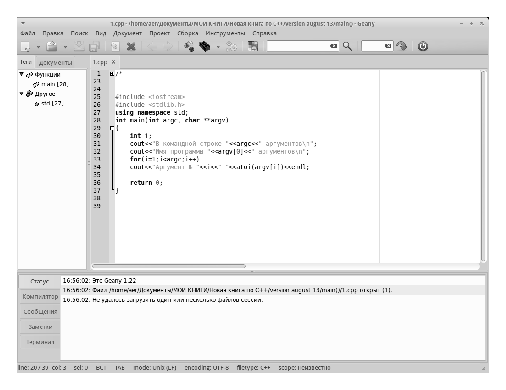
\includegraphics[width=0.7\textwidth]{img/ris_app_6}
\caption[Окно \Sys{Geany}.]{Окно \Sys{Geany}.}
\label{app:refDrawing5}
\end{center}
\end{figure}


Последовательно рассмотрим основные этапы разработки программы с использованием \Sys{Geany}. 
\begin{enumerate}
\item Необходимо создать шаблон приложения на \Sys{C/C++} (или другом языке программирования) с помощью 
команды \emph{Файл -> Создать из шаблона -> main.cxx}. После чего необходимо ввести текст 
программы и сохранить его. 
\item Для компиляции и запуска программы на выполнение служит пункт меню \emph{Сборка}. Для компиляции программы следует
использовать команду \emph{Сборка -> Скомпилировать} (\Sys{F8}). В этом случае будет построен объектный код программы (файл с расширением
\Sys{.o} или \Sys{.obj}). Для создания исполняемого кода программы служит команда \emph{Сборка -> Собрать} (\Sys{Shift+F9}).  Для
запуска программы следует выполнить команду \emph{Сборка -> Выполнить} (\Sys{F5}).
\end{enumerate}

Параметры компилятора определяются автоматически после выбора шаблона (\emph{Файл -> Создать из шаблона}).
Однако, команды компиляции и сборки по умолчанию можно изменить, используя команду \emph{Сборка -> Установить
параметры сборки} (см. рис.~\ref{app:refDrawing6}). Здесь \Sys{\%f} --- имя компилируемого файла, 
\Sys{\%e} --- имя файла без расширения.

\begin{figure}[htb]
\begin{center}
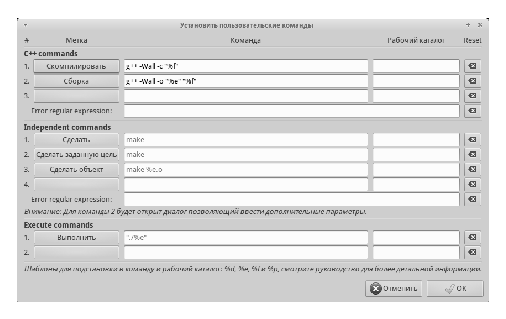
\includegraphics[width=0.7\textwidth]{img/ris_app_7}
\caption[Настройка компиляции программ на языке \Sys{C++} в \Sys{Geany}.]{Настройка компиляции программ на языке \Sys{C++} в
\Sys{Geany}.}
\label{app:refDrawing6}
\end{center}
\end{figure}

